\documentclass[11pt]{article}
\usepackage{graphicx}
\usepackage[left=2.00cm, right=2.00cm, top=2.00cm, bottom=2.00cm]{geometry}
\usepackage{amsmath}
\usepackage[colorlinks]{hyperref}
\usepackage[backend=biber]{biblatex}
\usepackage{eurosym}
\usepackage{subcaption}
\usepackage{accents}
\usepackage[capitalise]{cleveref}

\addbibresource{main.bib}
\graphicspath{{figures/}}

\crefname{relation}{Rel.}{Rels.}
\creflabelformat{relation}{(#2#1#3)}
\crefname{constraint}{Constr.}{Constrs.}
\creflabelformat{constraint}{(#2#1#3)}

\newcommand{\ubar}[1]{\underaccent{\bar}{#1}}


\newcommand{\generation}{g_{n,s,t}}
\newcommand{\generationpotential}{\bar{g}_{n,s,t}}
\newcommand{\capacityGeneration}{G_{n,s}}
\newcommand{\capacityFlow}{F_{\ell}}
\newcommand{\capexGeneration}{c_{n,s}}
\newcommand{\capexFlow}{c_{\ell}}
\newcommand{\opexGeneration}{o_{n,s}}
\newcommand{\demand}[1][n]{d_{#1,a,t}}
\newcommand{\utility}{U_{n,a,t}}
\newcommand{\incidence}{K_{n,\ell}}
\newcommand{\mulowergeneration}{\ubar{\mu}_{n,s,t}}
\newcommand{\muuppergeneration}{\bar{\mu}_{n,s,t}}
\newcommand{\mulowerflow}{\ubar{\mu}_{\ell,t}}
\newcommand{\muupperflow}{\bar{\mu}_{\ell,t}}
\newcommand{\lmp}[1][n]{\lambda_{#1,t}}
\newcommand{\flow}{f_{\ell,t}}

\newcommand{\allocatePeer}{A_{n \rightarrow m,t}}
\newcommand{\allocateFlow}{A_{n \rightarrow m,\ell,t}}
\newcommand{\allocateCapexGeneration}{\mathcal{C}^{G}_{m,t}}
\newcommand{\allocateCapexFlow}{\mathcal{C}^{F}_{m,t}}
\newcommand{\allocateOpex}{\mathcal{O}_{m,t}}
\newcommand{\allocateEmissionCost}{\mathcal{E}_{m,t}}

\newcommand{\emission}{e_{n,s}}
\newcommand{\emissionPrice}{\mu_{\text{CO2}}}
\newcommand{\megawatthour}{MWh$_\text{el}$}
\newcommand{\totalcost}{\mathcal{TC}}
\newcommand{\normedgeneration}{\tilde{g}_{n,s,t}}
\newcommand{\normeddemand}[1][n]{\tilde{d}_{#1,a,t}}
\newcommand{\impactcapexgeneration}{\Phi_{n,s,t}}
\newcommand{\impactcapexflow}{\Phi_{\ell,t}}
\newcommand{\resultsin}[1]{\hspace{20pt} \bot  \hspace{12pt} #1}
\newcommand{\Forall}[1]{\hspace{20pt} \forall \,\, #1}


\begin{document}


\title{From Flow Based Cost Allocation to Locational Marginal Prices}
\author{Fabian Hofmann}

\maketitle

% \begin{abstract}
% The abstract text goes here.
% \end{abstract}


\section*{Linear Energy Modelling and LMP}
We linearly optimize the capacity and dispatch of a simple power system. 

\begin{align}
    \underset{\demand, \generation, \capacityGeneration}{\text{max}}
    \left(\utility(\demand) - \sum_{n,s} \capexGeneration \capacityGeneration - \sum_{n, s, t} \opexGeneration \generation - \sum_{\ell} \capexFlow \, \capacityFlow \right) \label{eq:minisation}
\end{align}

where 
\begin{itemize}
\item[] $\utility$ denotes the utility function per bus $n$, demand type $a$ time step $t$ 
 \item[] $\demand$ denotes the eletric demand 
 \item[] $\capexGeneration$ denotes the capital expenditure (CAPEX) per node $n$ and generator type $s$
 \item[] $\capacityGeneration$ denotes the generation capacity
 \item[] $\opexGeneration$ denotes the operational cost (OPEX)
 \item[] $\generation$ denotes the net generation in MW
 \item[] $\capexFlow$ denotes the CAPEX per transmission line 
 \item[] $\capacityFlow$ denotes the transmission capacity.
\end{itemize}

\noindent
In the following we neglect the utility $\utility$ of the nodal demand while fixing the demand $\demand$ to a predefined time-series. The generation $\generation$ is constraint to its capacity
\begin{align}
 \generation - \generationpotential \capacityGeneration  &\le 0 \resultsin{\muuppergeneration}\Forall{n,s,t} 
 \label[constraint]{eq:upper_generation_capacity_constraint}\\ 
 - \generation &\le 0 \resultsin{\mulowergeneration} \Forall{n,s,t} 
 \label[constraint]{eq:lower_generation_capacity_constraint}
 \end{align}
where $\generationpotential \in \left[ 0,1\right]$ is the capacity factor for renewable generators. The constraints yield the KKT variables $\muuppergeneration$ and $\mulowergeneration$ which due to complementary slackness are only non-zero if the corresponding constraint is binding. 

\noindent
The transmission capacity $\capacityFlow$ limits the flow $\flow$ in both directions, such that 
\begin{align}
 \flow - \capacityFlow \le 0 \resultsin{\muupperflow} \Forall{\ell,t} 
 \label[constraint]{eq:upper_flow_capacity_constraint} \\
 - \flow - \capacityFlow \le 0 \resultsin{\mulowerflow} \Forall{\ell,t} 
 \label[constraint]{eq:lower_flow_capacity_constraint}
\end{align}
The yielding KKT variables $\muupperflow$ and $\mulowerflow$ are only non-zero if $\flow$ is limited by the trasmission capacity in positive or negative direction, i.e. \cref{eq:upper_flow_capacity_constraint} or \cref{eq:lower_flow_capacity_constraint} are binding. \\

The nodal balance constraint ensures that the amount of power that flows into a bus equals the power that flows out of a bus, thus reflects the Kirchhoff Current Law (KCL)
\begin{align}
    \sum_s \generation - \sum_a \demand - \sum_l \incidence \, \flow = 0 \resultsin{\lmp} \Forall{n,t}
    \label[constraint]{eq:nodal_balance_lin}
\end{align}
Its shadow price mirrors the Locational Marginal Prizes (LMP) $\lmp$ per bus and time step. In a power market this is the \euro/\megawatthour-price which a consumer has to pay. \\

As the shown in \cite{brown_decreasing_2020}, the OPEX and CAPEX of generators follow the non-profit rule which states that their expenses equals their total revenue 

\begin{align}
\capexGeneration \, \capacityGeneration + \sum_{t} \opexGeneration \, \generation = \sum_{t} \lmp \, \generation \Forall{n,s}\label{eq:non_profit_generator}
\end{align}

\noindent
The relation counts for transmission lines where the CAPEX amounts to the total congestion revenue
\begin{align}
\capexFlow \, \capacityFlow = \sum_{n,t} \lmp \, \incidence \, \flow \Forall{\ell} \label{eq:non_profit_branch}
\end{align}
Note that we are neglecting the Kirchhoff Voltage Law (KVL) constraints. Finally, the total cost $\totalcost$, consisting of all CAPEX and OPEX have to be payed by the consumers 

\begin{align}
\totalcost = \sum_{n,s} \capexGeneration \, \capacityGeneration + \sum_{n,s,t} \opexGeneration \, \generation + \sum_{\ell} \capexFlow \, \capacityFlow = \sum_{n,a,t} \lmp \, \demand 
\label{eq:total_system_cost}
\end{align}


\subsection*{Adding CO$_2$ Constraints}

Imposing an additional CO$_2$ constraint limiting the total emission to K,  
\begin{align}
 \sum_{n,s,t} \emission \, \generation \le \text{K} \resultsin{\emissionPrice} 
 \label[constraint]{eq:co2_constraint}
\end{align}
with $\emission$ being the emission factor in tonne-CO$_2$ per \megawatthour, returns an effective CO$_2$ price $\emissionPrice$ in \euro/tonne-CO$_2$. The CO$_2$ price shifts the right hand side of the non-profit relation for generators \cref{eq:non_profit_generator} to

\begin{align}
\capexGeneration \, \capacityGeneration + \sum_{t} \opexGeneration \, \generation = \sum_{t} \left( \lmp - \emission \, \emissionPrice \right)  \, \generation \Forall{n,s} 
\label{eq:non_profit_generator_emission}
\end{align}
This shows nicely the duality for exchanging the CO$_2$ \cref{eq:co2_constraint} for a shifted OPEX which includes the CO$_2$ costs

\begin{align}
\opexGeneration \rightarrow \opexGeneration + \emission \, \emissionPrice \label[relation]{eq:shift_opex_by_emission_cost}
\end{align}

% ----------------------------------------------------------------------------------------
% ----------------------------------------------------------------------------------------

\section*{Flow Based Cost Allocation}

Besides using LMP, there are others methods for distributing costs in a power system. A common approach is based on Flow Allocation (FA) methods which determine peer-to-peer (P2P) relations between producers (sources) and consumers (sinks) and thus enable to directly assign costs to the consumers. %Due to the non-determnistic tracing of power through the network the methods result in different allocation. 
Let $\allocatePeer$ denotes the power that is produced at bus $n$ at time $t$ and assigned to consumers at bus $m$. We will refer to it as a P2P relation between $n$ and $m$. Further let $\allocateFlow$ denote flow on line $\ell$ at time $t$ caused by the P2P connection $n\rightarrow m$.\\
\noindent
In the following we show how the LMP can be reproduced on the basis of FA. 

\subsubsection*{Allocating Operational Expenditures}
Consumers at bus $m$ compensate the OPEX proportionally to the assigned production, thus 
\begin{align}
\allocateOpex = \sum_{n,s} \opexGeneration \, \normedgeneration \, \allocatePeer \Forall{m,t} \label{eq:allocate_opexGeneration}
\end{align}
where $\normedgeneration = \generation/\sum_s \generation$ denotes the share of generator $s$ of the nodal production. \\

\subsubsection*{Allocating CO$_2$ Cost}
 Similar to the OPEX (compare \cref{eq:shift_opex_by_emission_cost}) consumers at bus $m$ compensate the CO$_2$ cost, thus 
\begin{align}
 \allocateEmissionCost = \sum_{n,s} \emissionPrice \, \emission \, \normedgeneration \, \allocatePeer \Forall{m,t} \label{eq:allocate_emissionPrice}
\end{align}


\subsubsection*{Allocating Capital Expenditures for Generators}
According to the polluter pays principle, the CAPEX allocation should differentiate between consumers who are `responsible` for investments and those who are not. Thus, it is crucial to know whether a time step $t$ makes investments in $\capacityGeneration$ necessary or if it would be feasible without (further) investments. The KKT variable of the upper generator capacity constraint $\muuppergeneration$ gives us the needed estimator: If $\muuppergeneration > 0$, the upper capacity constraint \cref{eq:upper_generation_capacity_constraint} is binding and it can be fairly assumed that these times steps cause investments in $\capacityGeneration$. If in contrast $\muuppergeneration = 0$, the generation $\generation$ is not bound and does not push further investments in $\capacityGeneration$.
On the basis of the KKT variable $\muuppergeneration$ we are able to define a measure $\impactcapexgeneration$ for the impact on the investments in $\capacityGeneration$  
\begin{align}
    \impactcapexgeneration = \dfrac{\muuppergeneration}{\sum_t \muuppergeneration \, \generation}
\end{align}
which weights the contributions of consumers at bus $m$ at time $t$ to the CAPEX 
\begin{align}
    \allocateCapexGeneration = \sum_{n,s} \capexGeneration \, \capacityGeneration \, \impactcapexgeneration\, \allocatePeer \Forall{m,t} \label{eq:allocate_capexGeneration}
\end{align}

\noindent
If consumers at $m$ retrieve power from $n$ when $\impactcapexgeneration$ is large, their contribution to investments in $\capacityGeneration$ raises. On the other hand, if consumers at $m$ retrieve power from $n$ when $\impactcapexgeneration=0$ , their contribution to $\capacityGeneration$ remain unchanged. 

\noindent
\textit{Side note}: A way more simple approach would neglect these thoughts and let  consumers at $m$ compensate CAPEX for generator $s$ at bus $n$ proportional to their retrieved power. This would lead us to $ \impactcapexgeneration = \left( \generation\right)^{-1}$. 

\subsubsection*{Allocating Capital Expenditures for Transmission Lines}
The allocation of CAPEX per the transmission line $\capexFlow \, \capacityFlow $ follows a similar procedure as for the generators. Again, we build up on KKT variables $\muupperflow$ and $\mulowerflow$ which translate to the necessity of transmission expansion of $\ell$ at time $t$. The measure $\impactcapexflow$ respects the need of CAPEX of both flow directions when set to 

\begin{align}
    \impactcapexflow = \dfrac{\muupperflow + \mulowerflow}{\sum_t \left( \muupperflow + \mulowerflow \right) \, \flow}
\end{align}

and weights the contributions of consumers at bus $m$ at time $t$ to the CAPEX in line $\ell$,
\begin{align}
    \allocateCapexFlow = \sum_{n,\ell} \capexFlow \, \capacityFlow\, \impactcapexflow, \allocateFlow \Forall{m,t} \label{eq:allocate_capexFlow}
\end{align}

\subsubsection*{Reproducing the LMP Based Consumption Costs}
The above presented quantities complete an allocation of the total cost $\totalcost$ which mirrors the cost allocation based on LMP, thus 

\begin{align}
 \allocateOpex + \allocateEmissionCost + \allocateCapexGeneration + \allocateCapexFlow \simeq \lmp[m] \, \demand[m] \Forall{m,t} 
 \label{eq:allocated_cost_mirror_lmp}
\end{align}



\subsection*{play around}



\section*{Showcase}

\subsection*{Network with CO$_2$ constraint}
We illustrate the flow based cost allocation under use of the fictive network shown in \cref{fig:network}. It consists of nine buses and ten time steps. The solver optimizes the capacity of two generators, wind and gas, per bus. ...   

\begin{figure}[h]
    \centering
    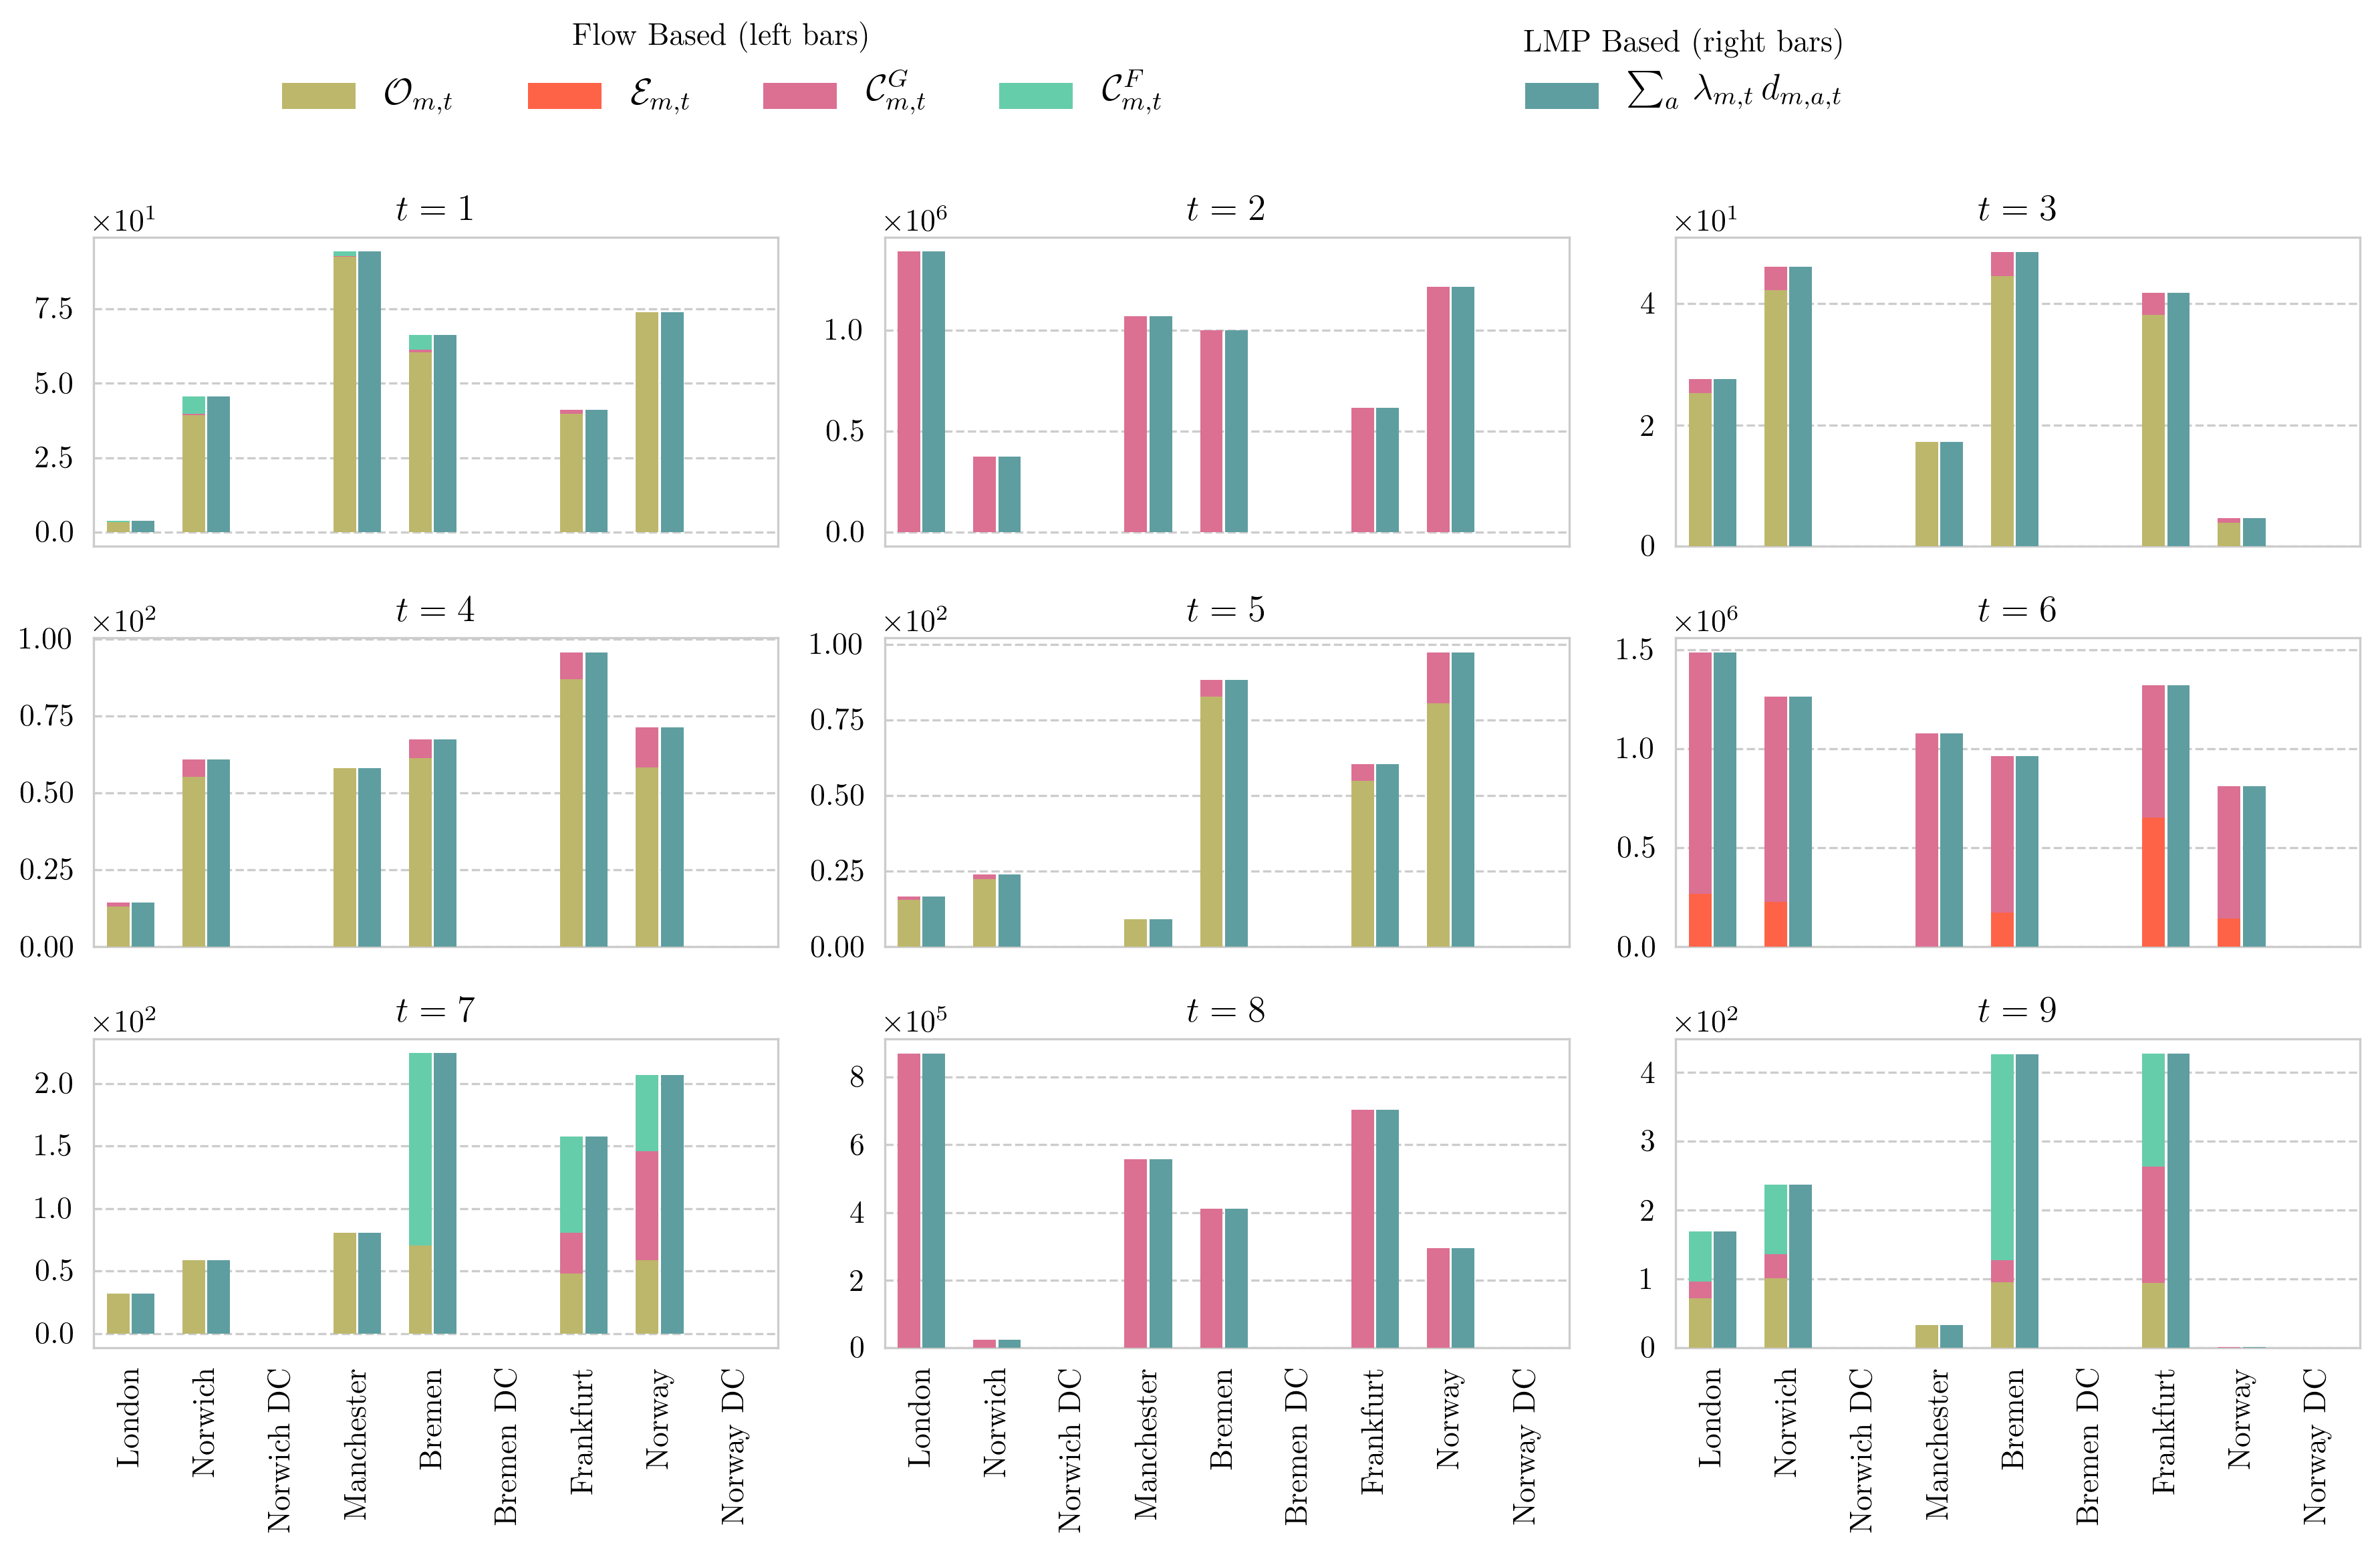
\includegraphics[width=\textwidth]{compare_allocation.png}
    \caption{Comparison of the stacked flow based cost allocation with the LMP based cost per consumer for each time step $t$ without CO$_2$ constaint. The left bars consist of the allocated OPEX $\allocateOpex$, the allocated CO$_2$ cost $\allocateEmissionCost$, the allocated generator CAPEX $\allocateCapexGeneration$ and transmission CAPEX $\allocateCapexFlow$, while the right bars show the of the nodal consumption times the LMP. }
    \label{fig:cost_allocation}
\end{figure}

\begin{figure}[h]
\begin{subfigure}{.5\textwidth}
\centering
 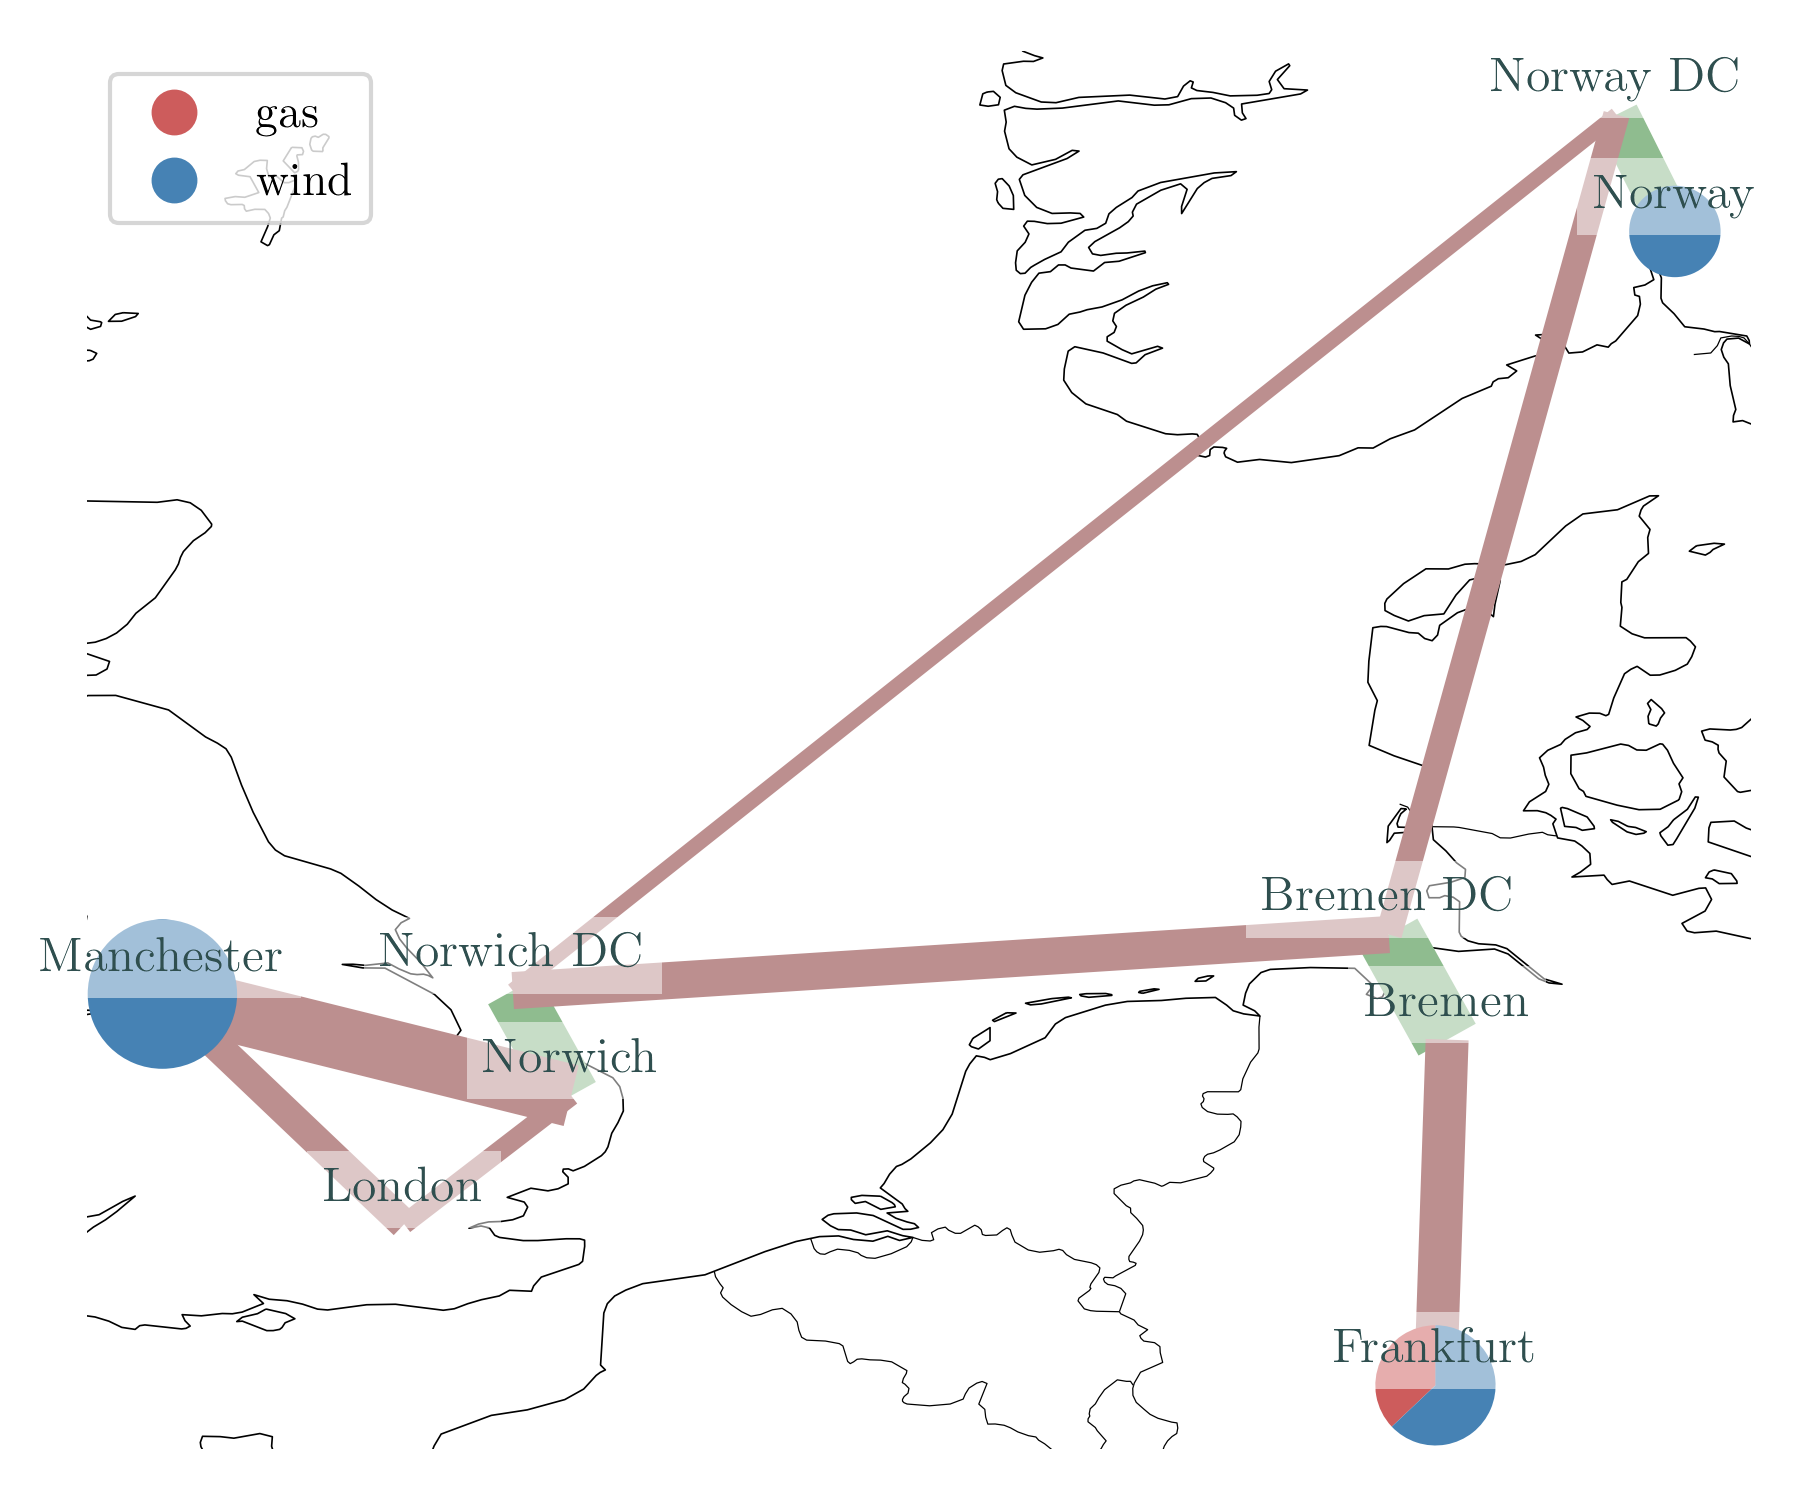
\includegraphics[width=\textwidth]{network.png}
 \caption{}
 \label{fig:network}
\end{subfigure}
\begin{subfigure}{.5\textwidth}   
    \centering
    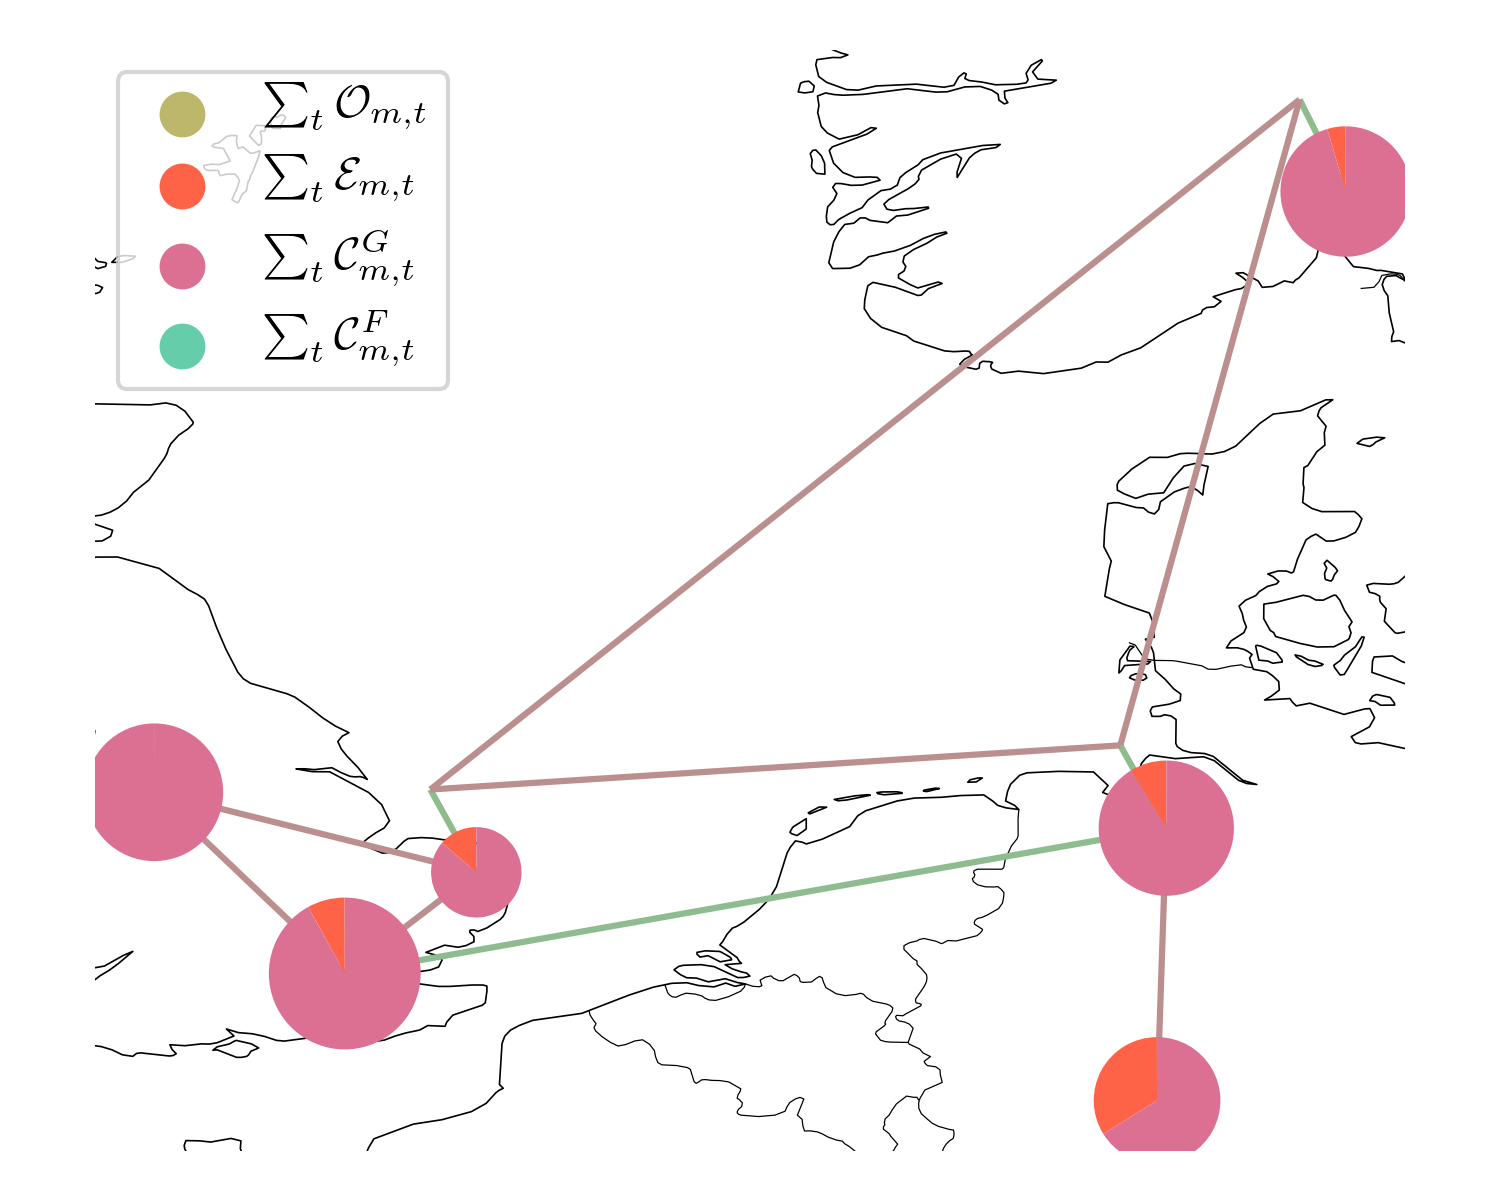
\includegraphics[width=\textwidth]{nodal_payments.png}
    \caption{}
    \label{fig:nodal_payments}
\end{subfigure}
\caption{Network used for showcasing. (a) shows the distributing of generation capacities $\capacityGeneration$, the widths of the transmission lines are proportional to their thermal limit $\capacityFlow$. (b) shows the total nodal payments according to the cost allocation.}
\end{figure}





\newpage
\subsubsection*{Relaxed CO$_2$ Constraint}


\begin{figure}[h]
\begin{subfigure}{.5\textwidth}
\centering
 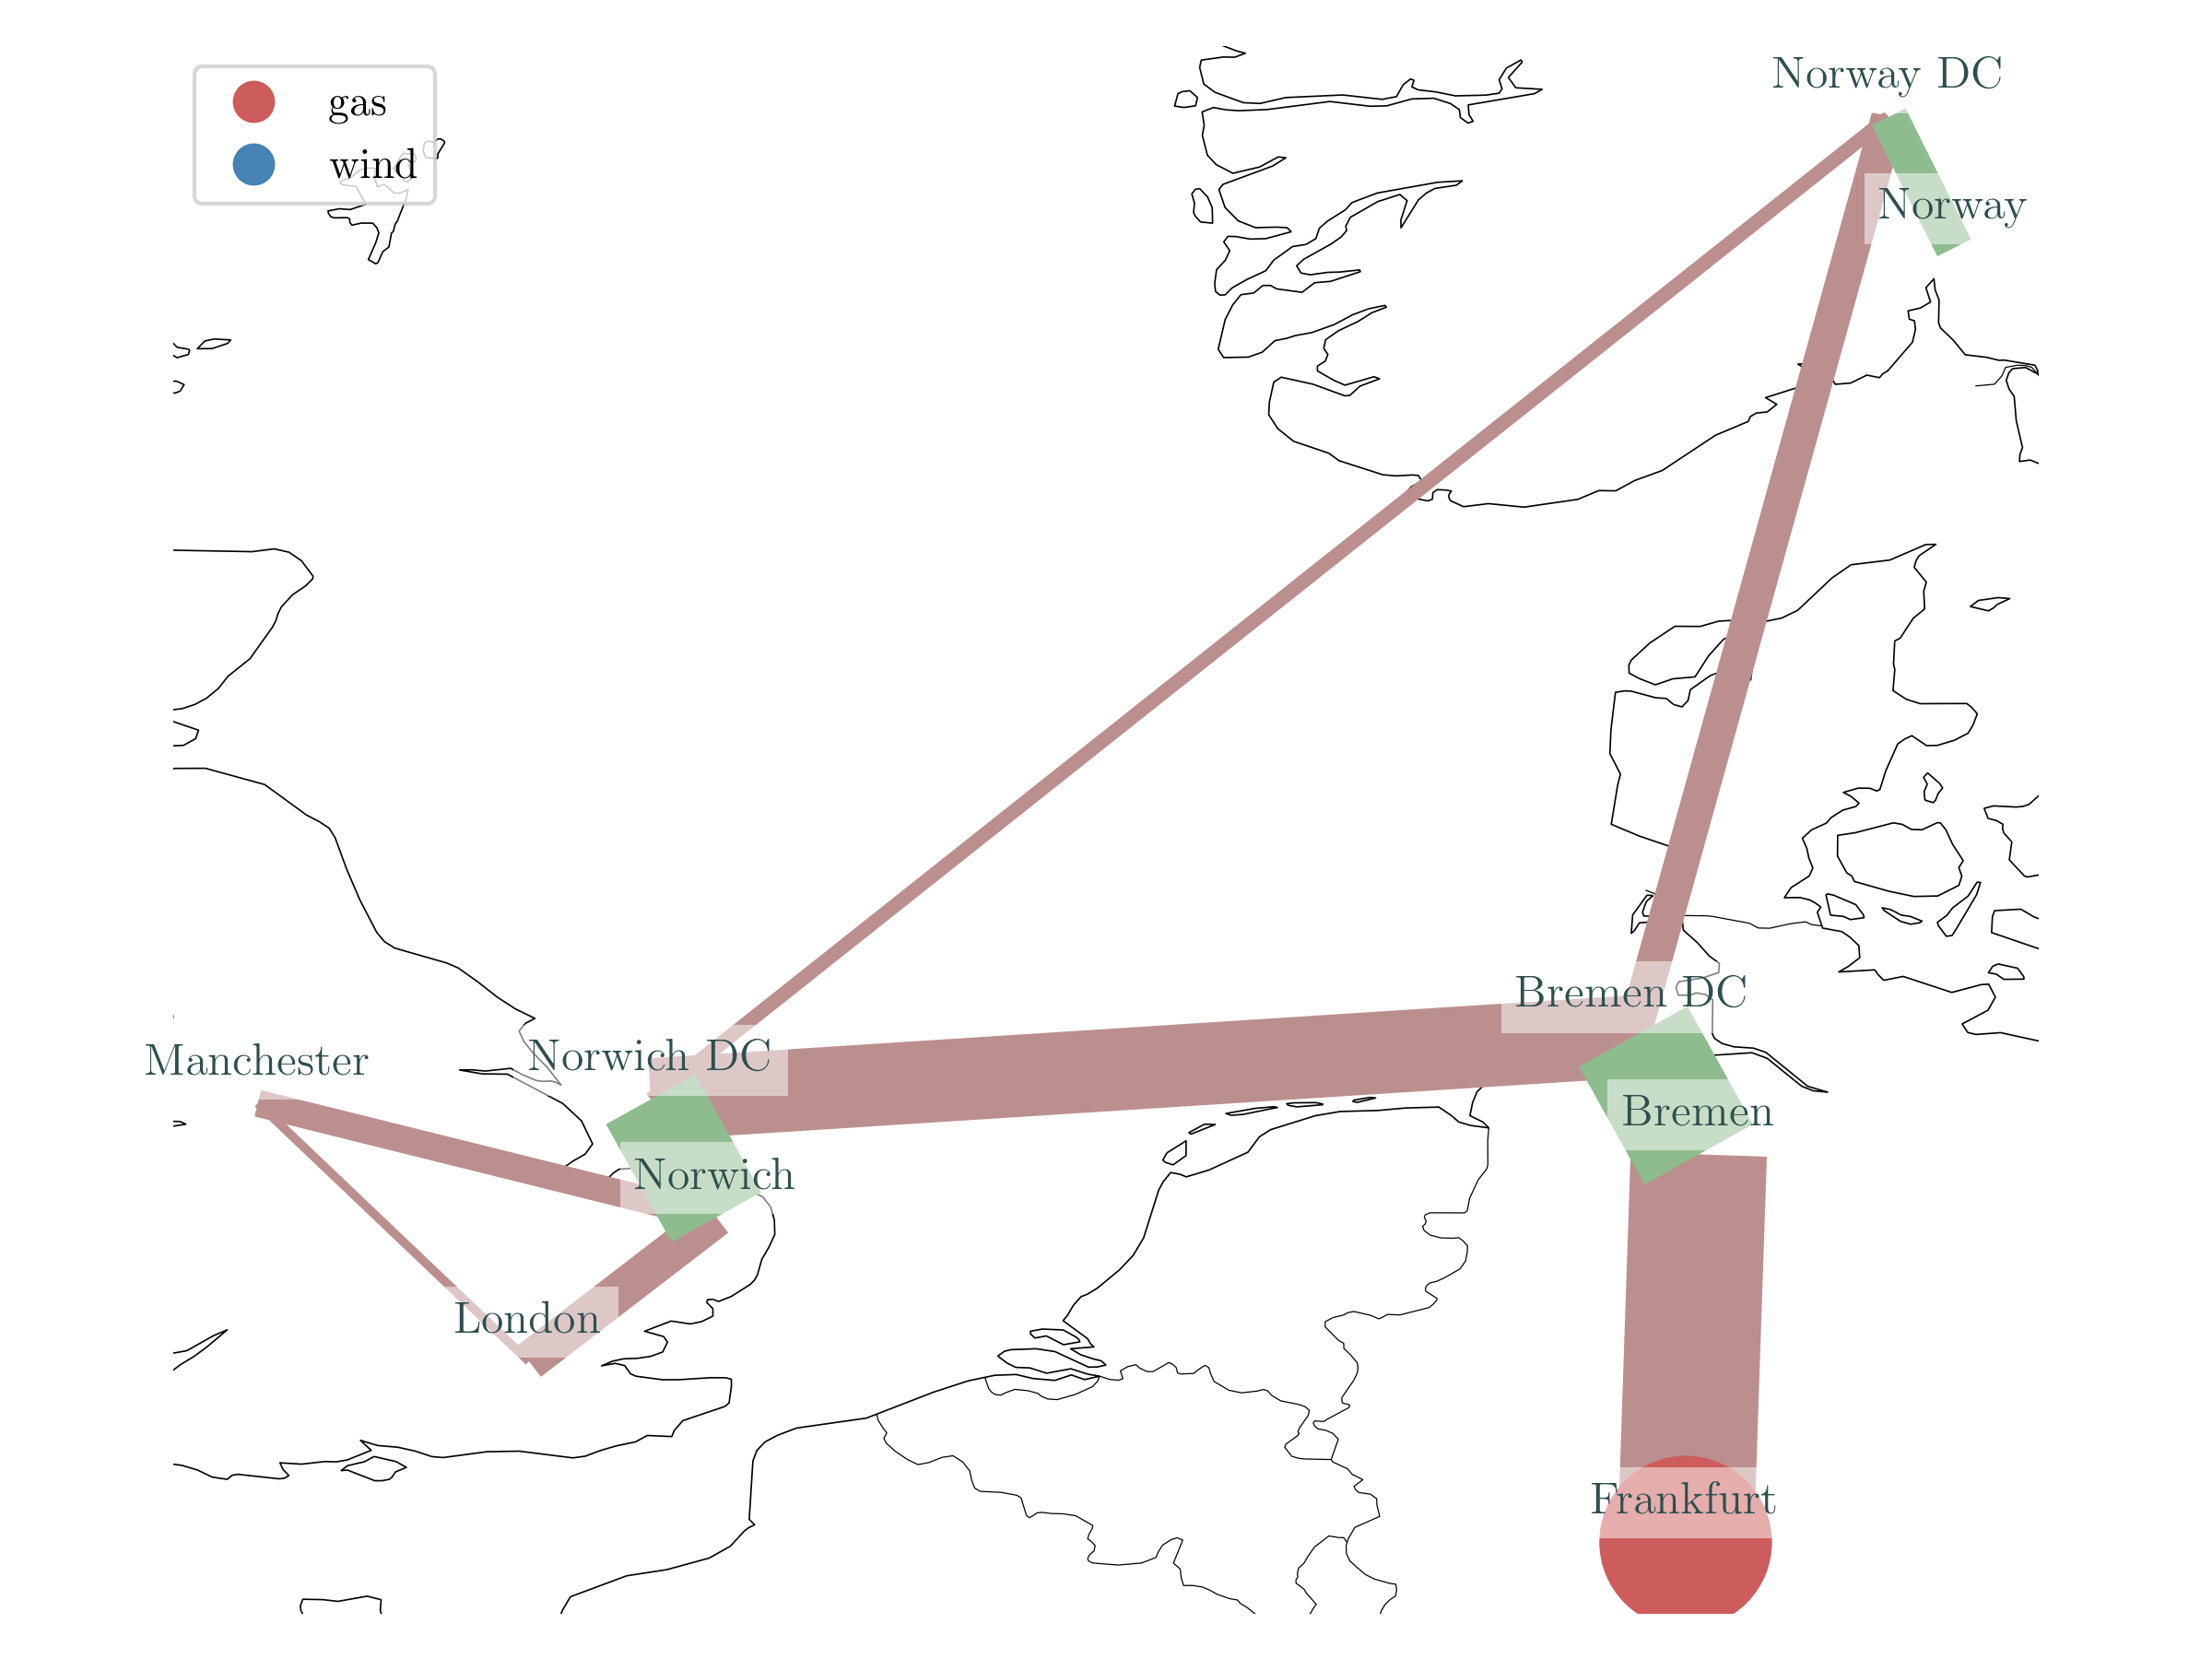
\includegraphics[width=\textwidth]{network_relaxed_co2.png}
 \caption{}
 \label{fig:network_relaxed_co2}
\end{subfigure}
\begin{subfigure}{.5\textwidth}   
    \centering
    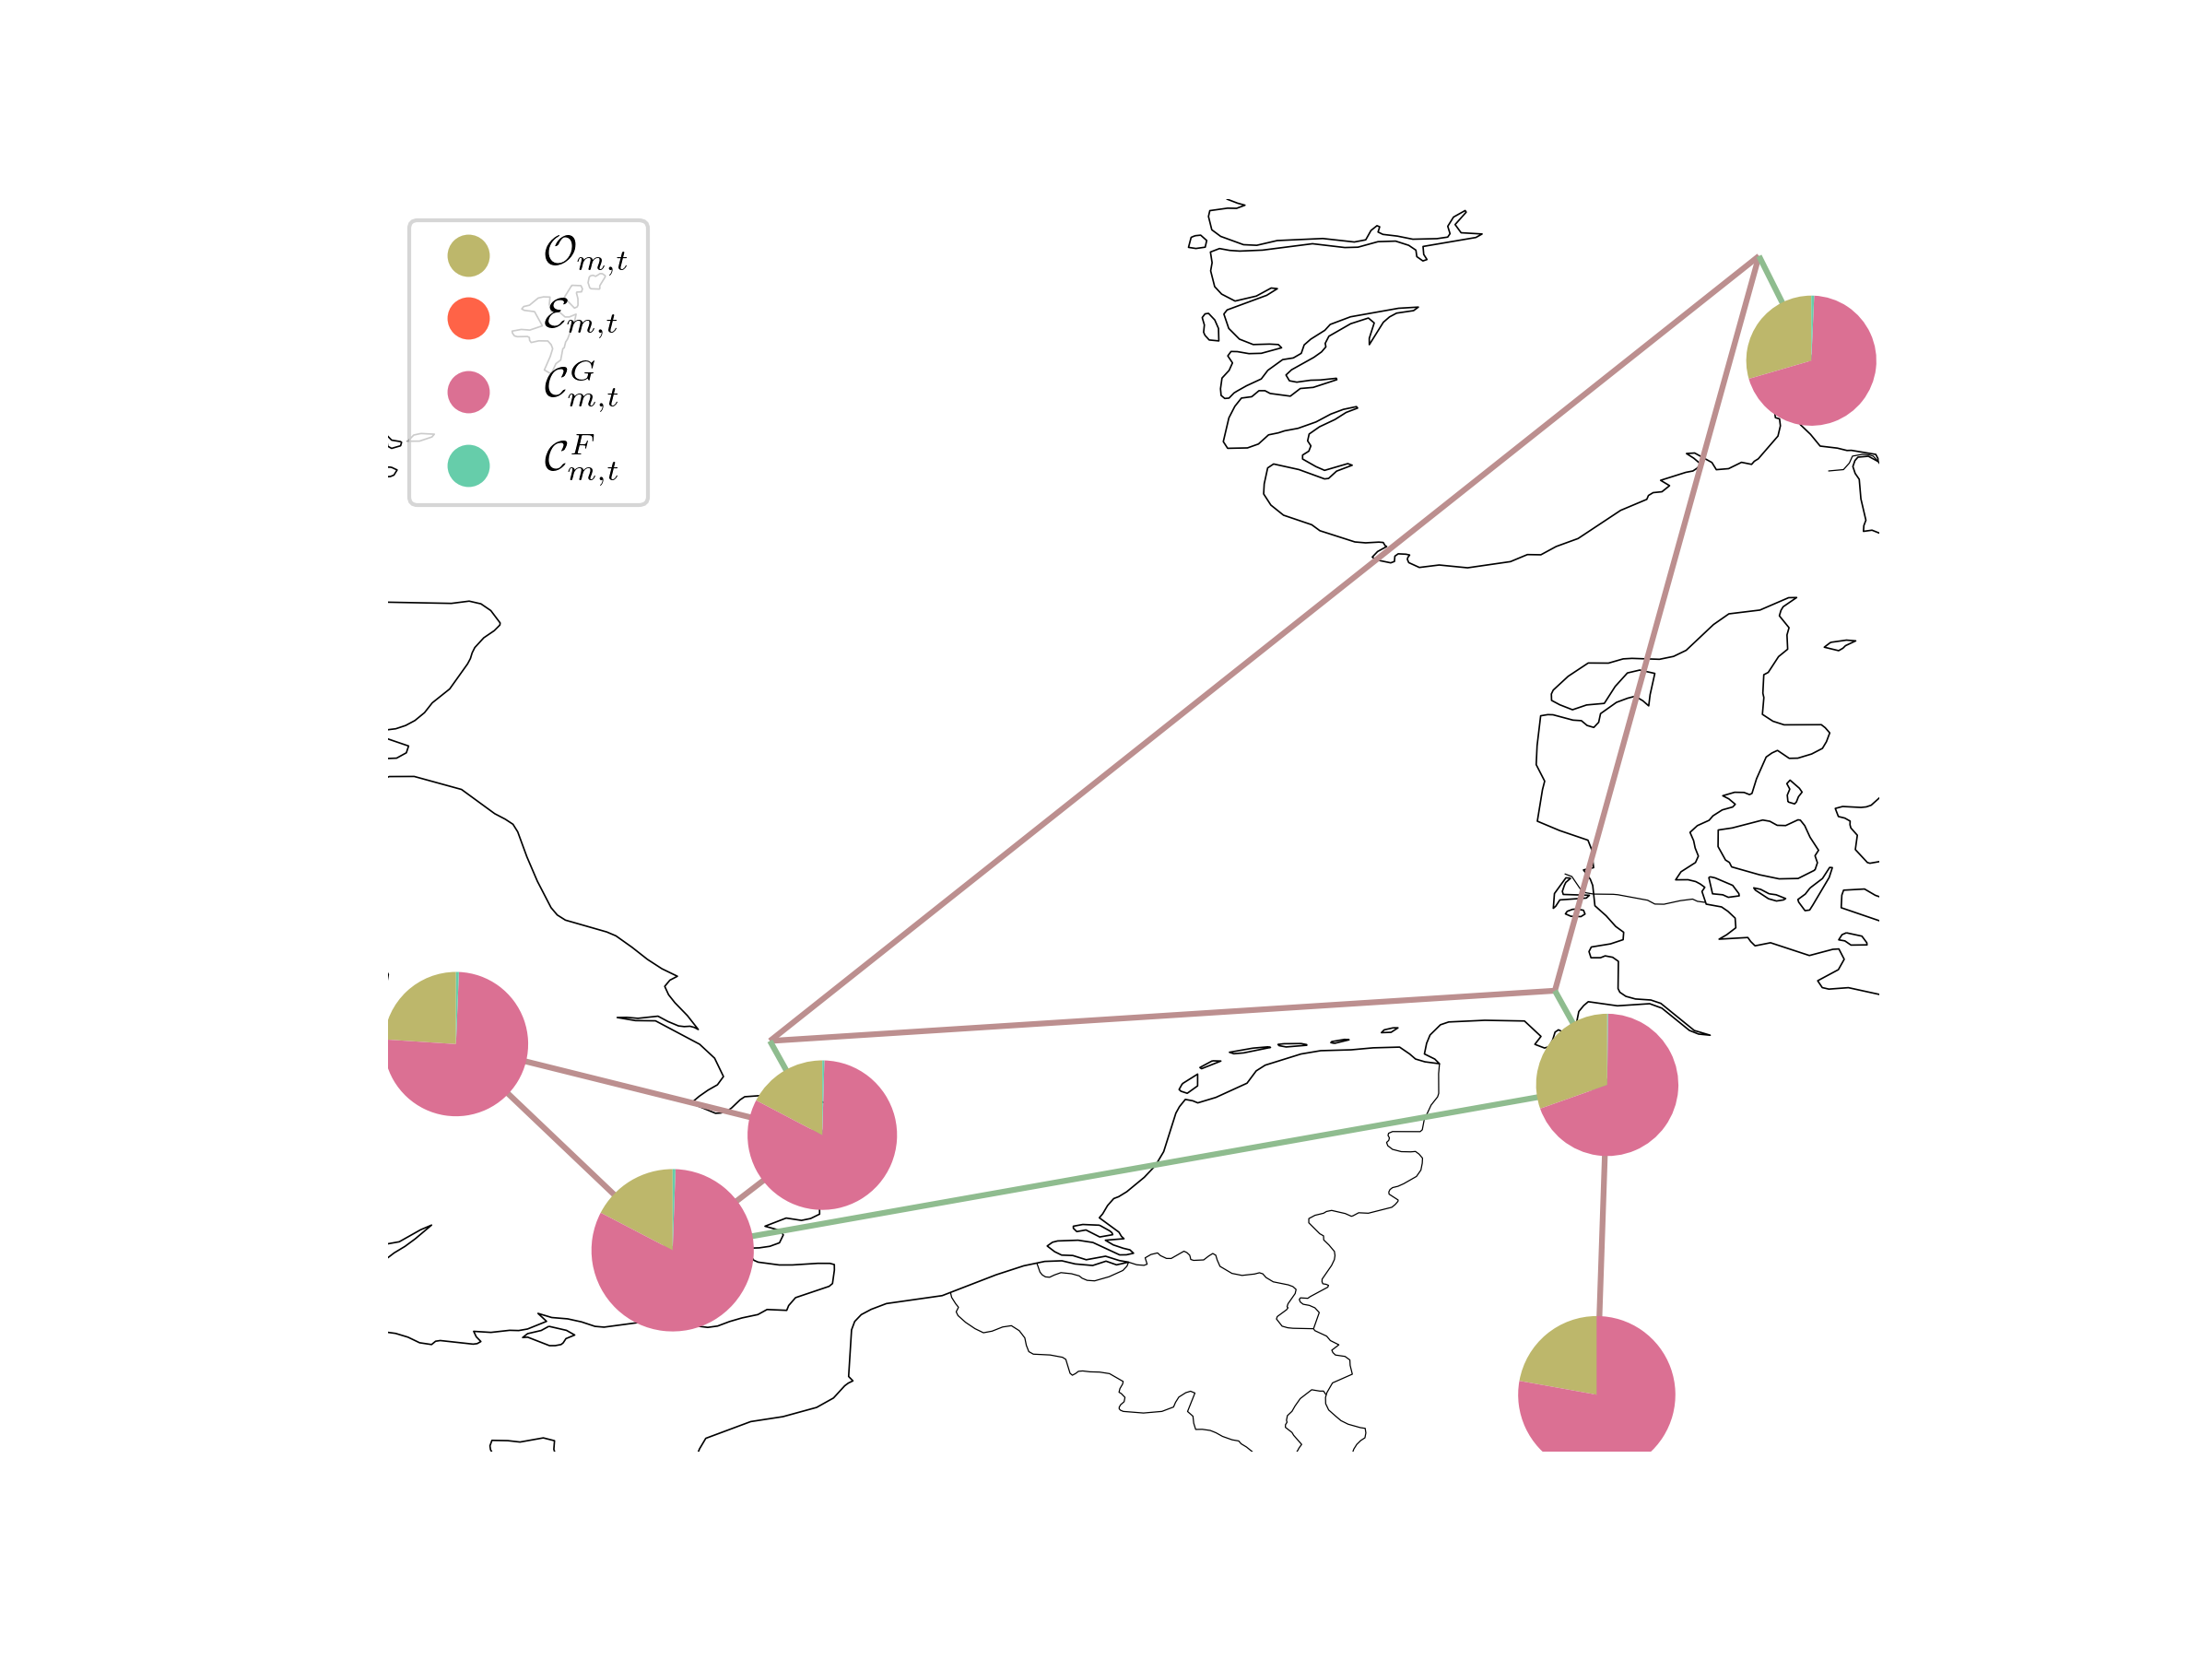
\includegraphics[width=\textwidth]{nodal_payments_relaxed_co2.png}
    \caption{}
    \label{fig:nodal_payments_relaxed_co2}
\end{subfigure}
\caption{Similar to \cref{fig:network} and \cref{fig:nodal_payments} but without CO$_2$ constraint.}
\end{figure}

\begin{figure}[h]
    \centering
    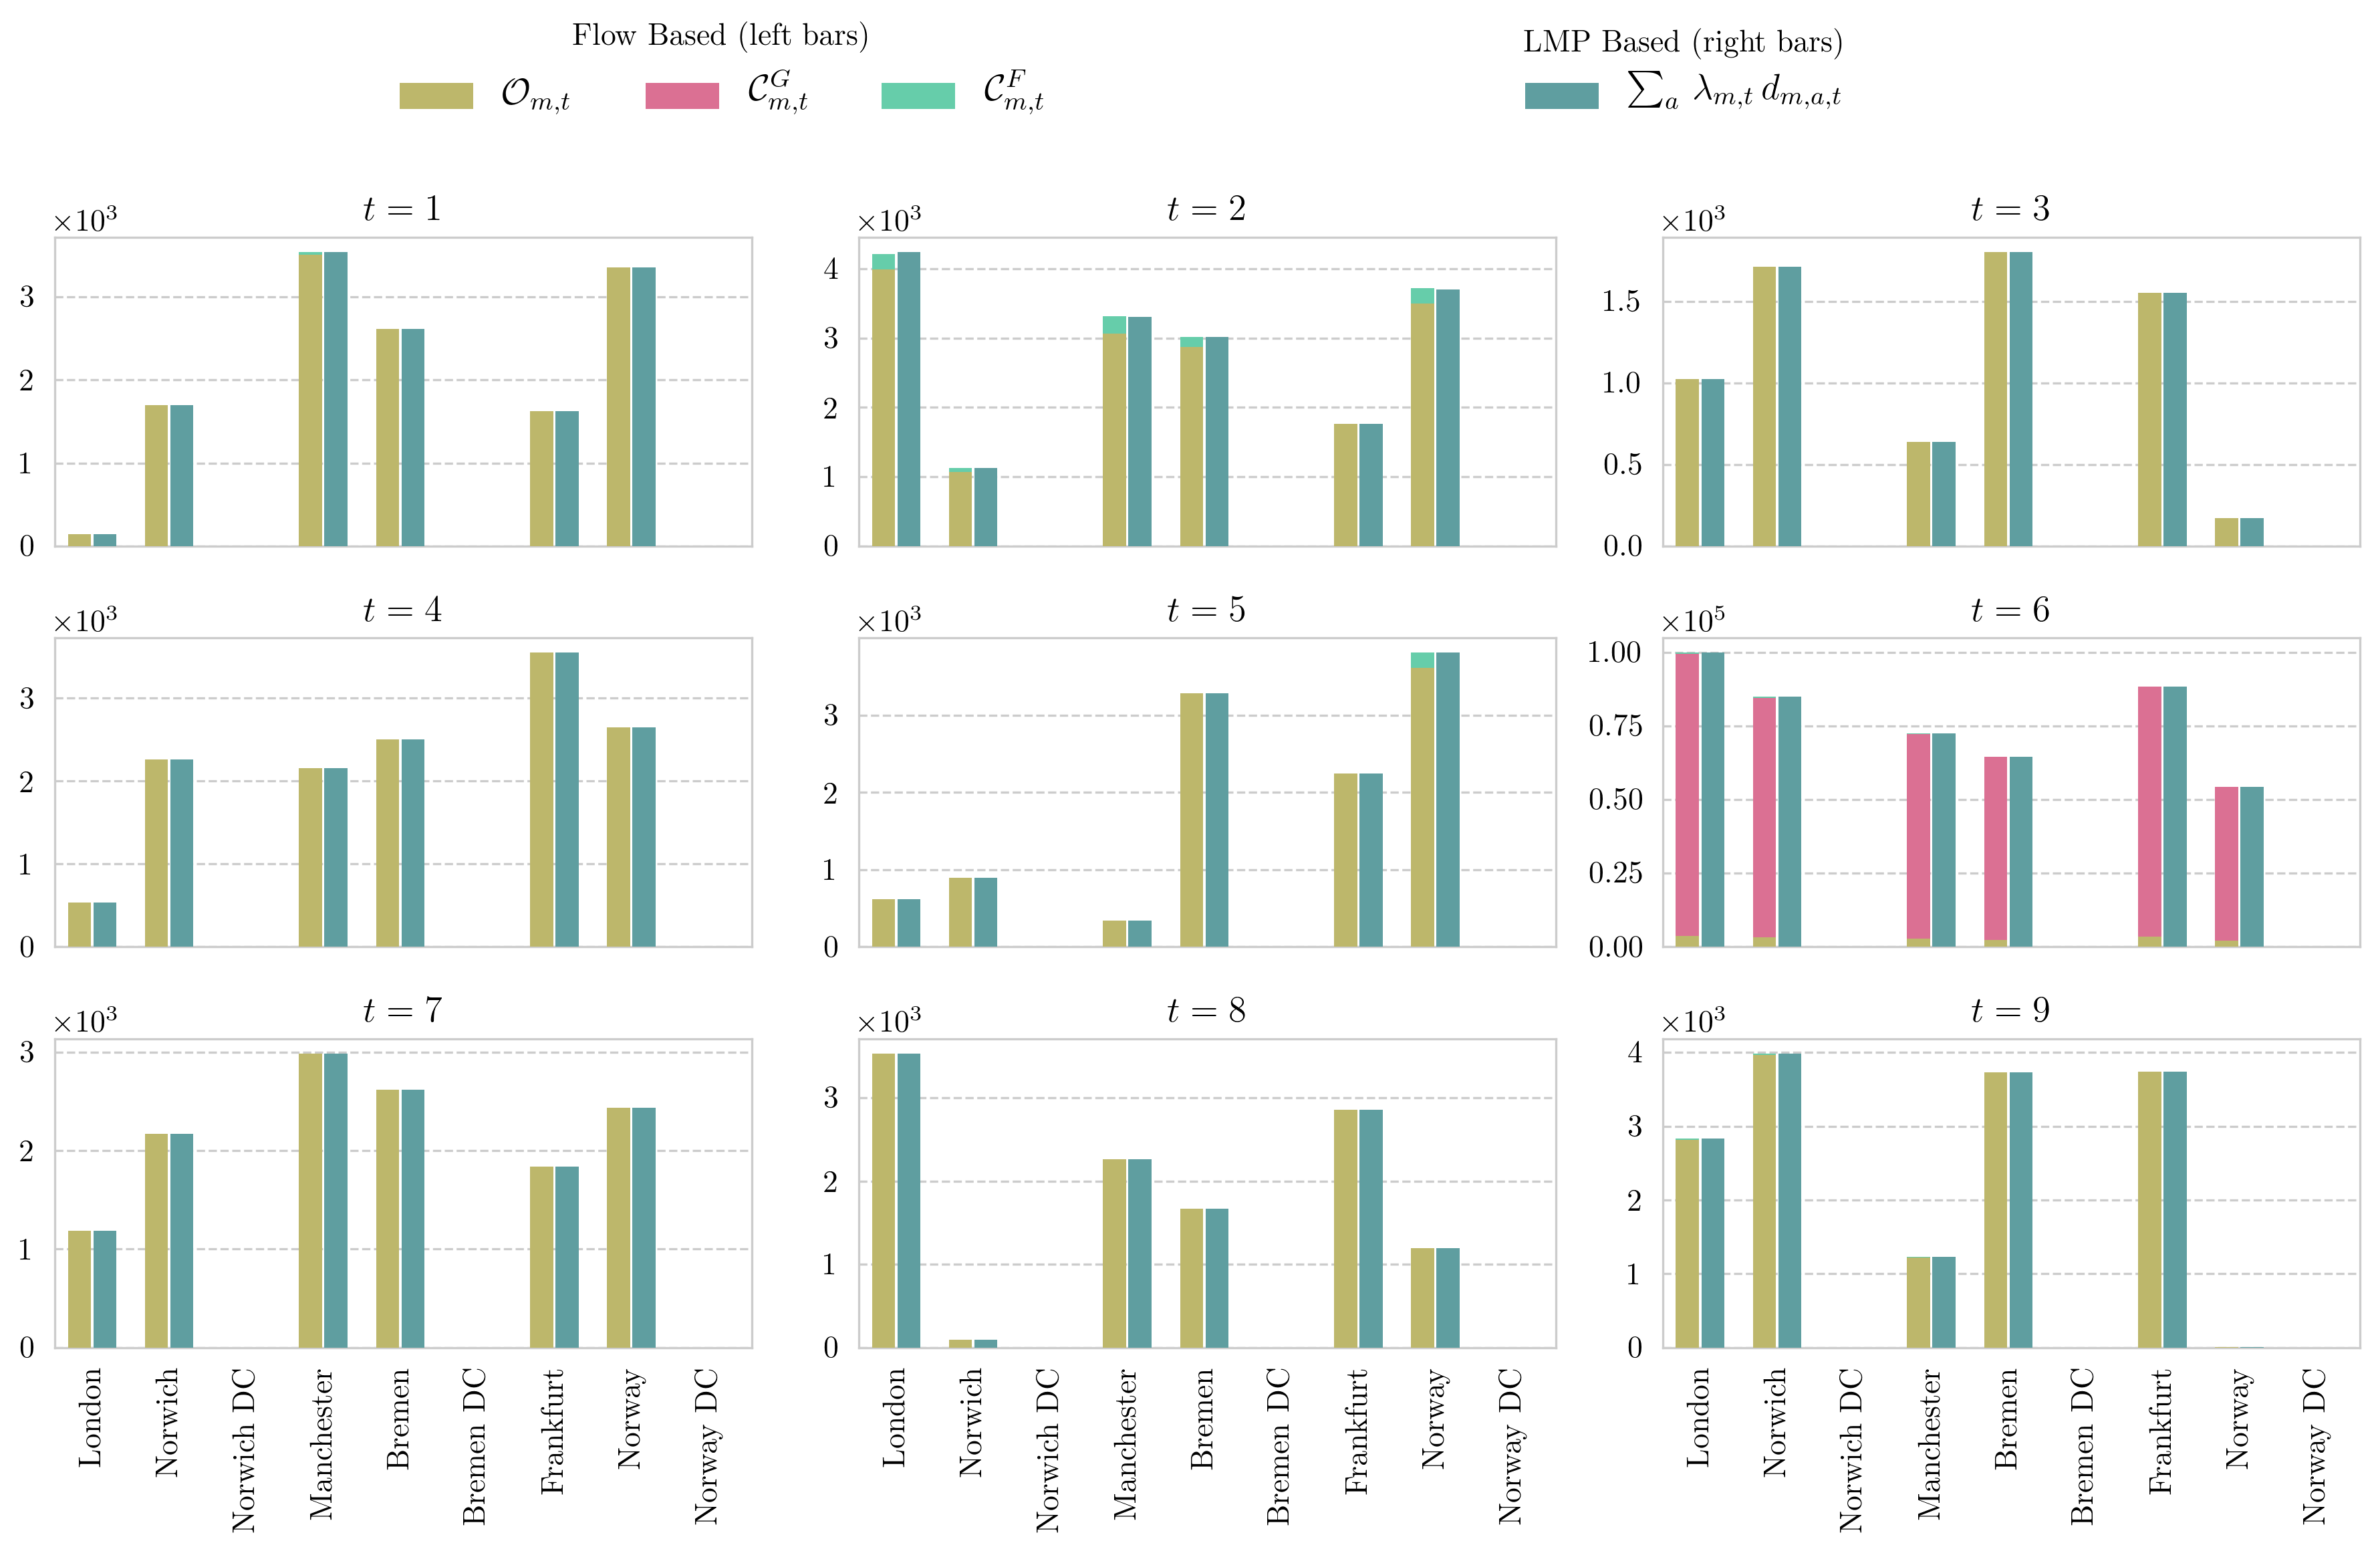
\includegraphics[width=\textwidth]{compare_allocation_relaxed_co2.png}
    \caption{Comparison of the stacked flow based cost allocation with the LMP based cost per consumer for each time step $t$ without CO$_2$ \cref{eq:co2_constraint}. Only one time-step $t=6$ determines the allocation of generator CAPEX $\allocateCapexGeneration$, as for all other time-steps \cref{eq:upper_generation_capacity_constraint} is not binding. Again note the cost scale difference between time step 6 and all others.}
    \label{fig:cost_allocation}
\end{figure}

% \subsection*{How does the cost flow through the network}
% 
% \begin{figure}[h]
%     \begin{subfigure}{.5\textwidth}
%       \centering
%       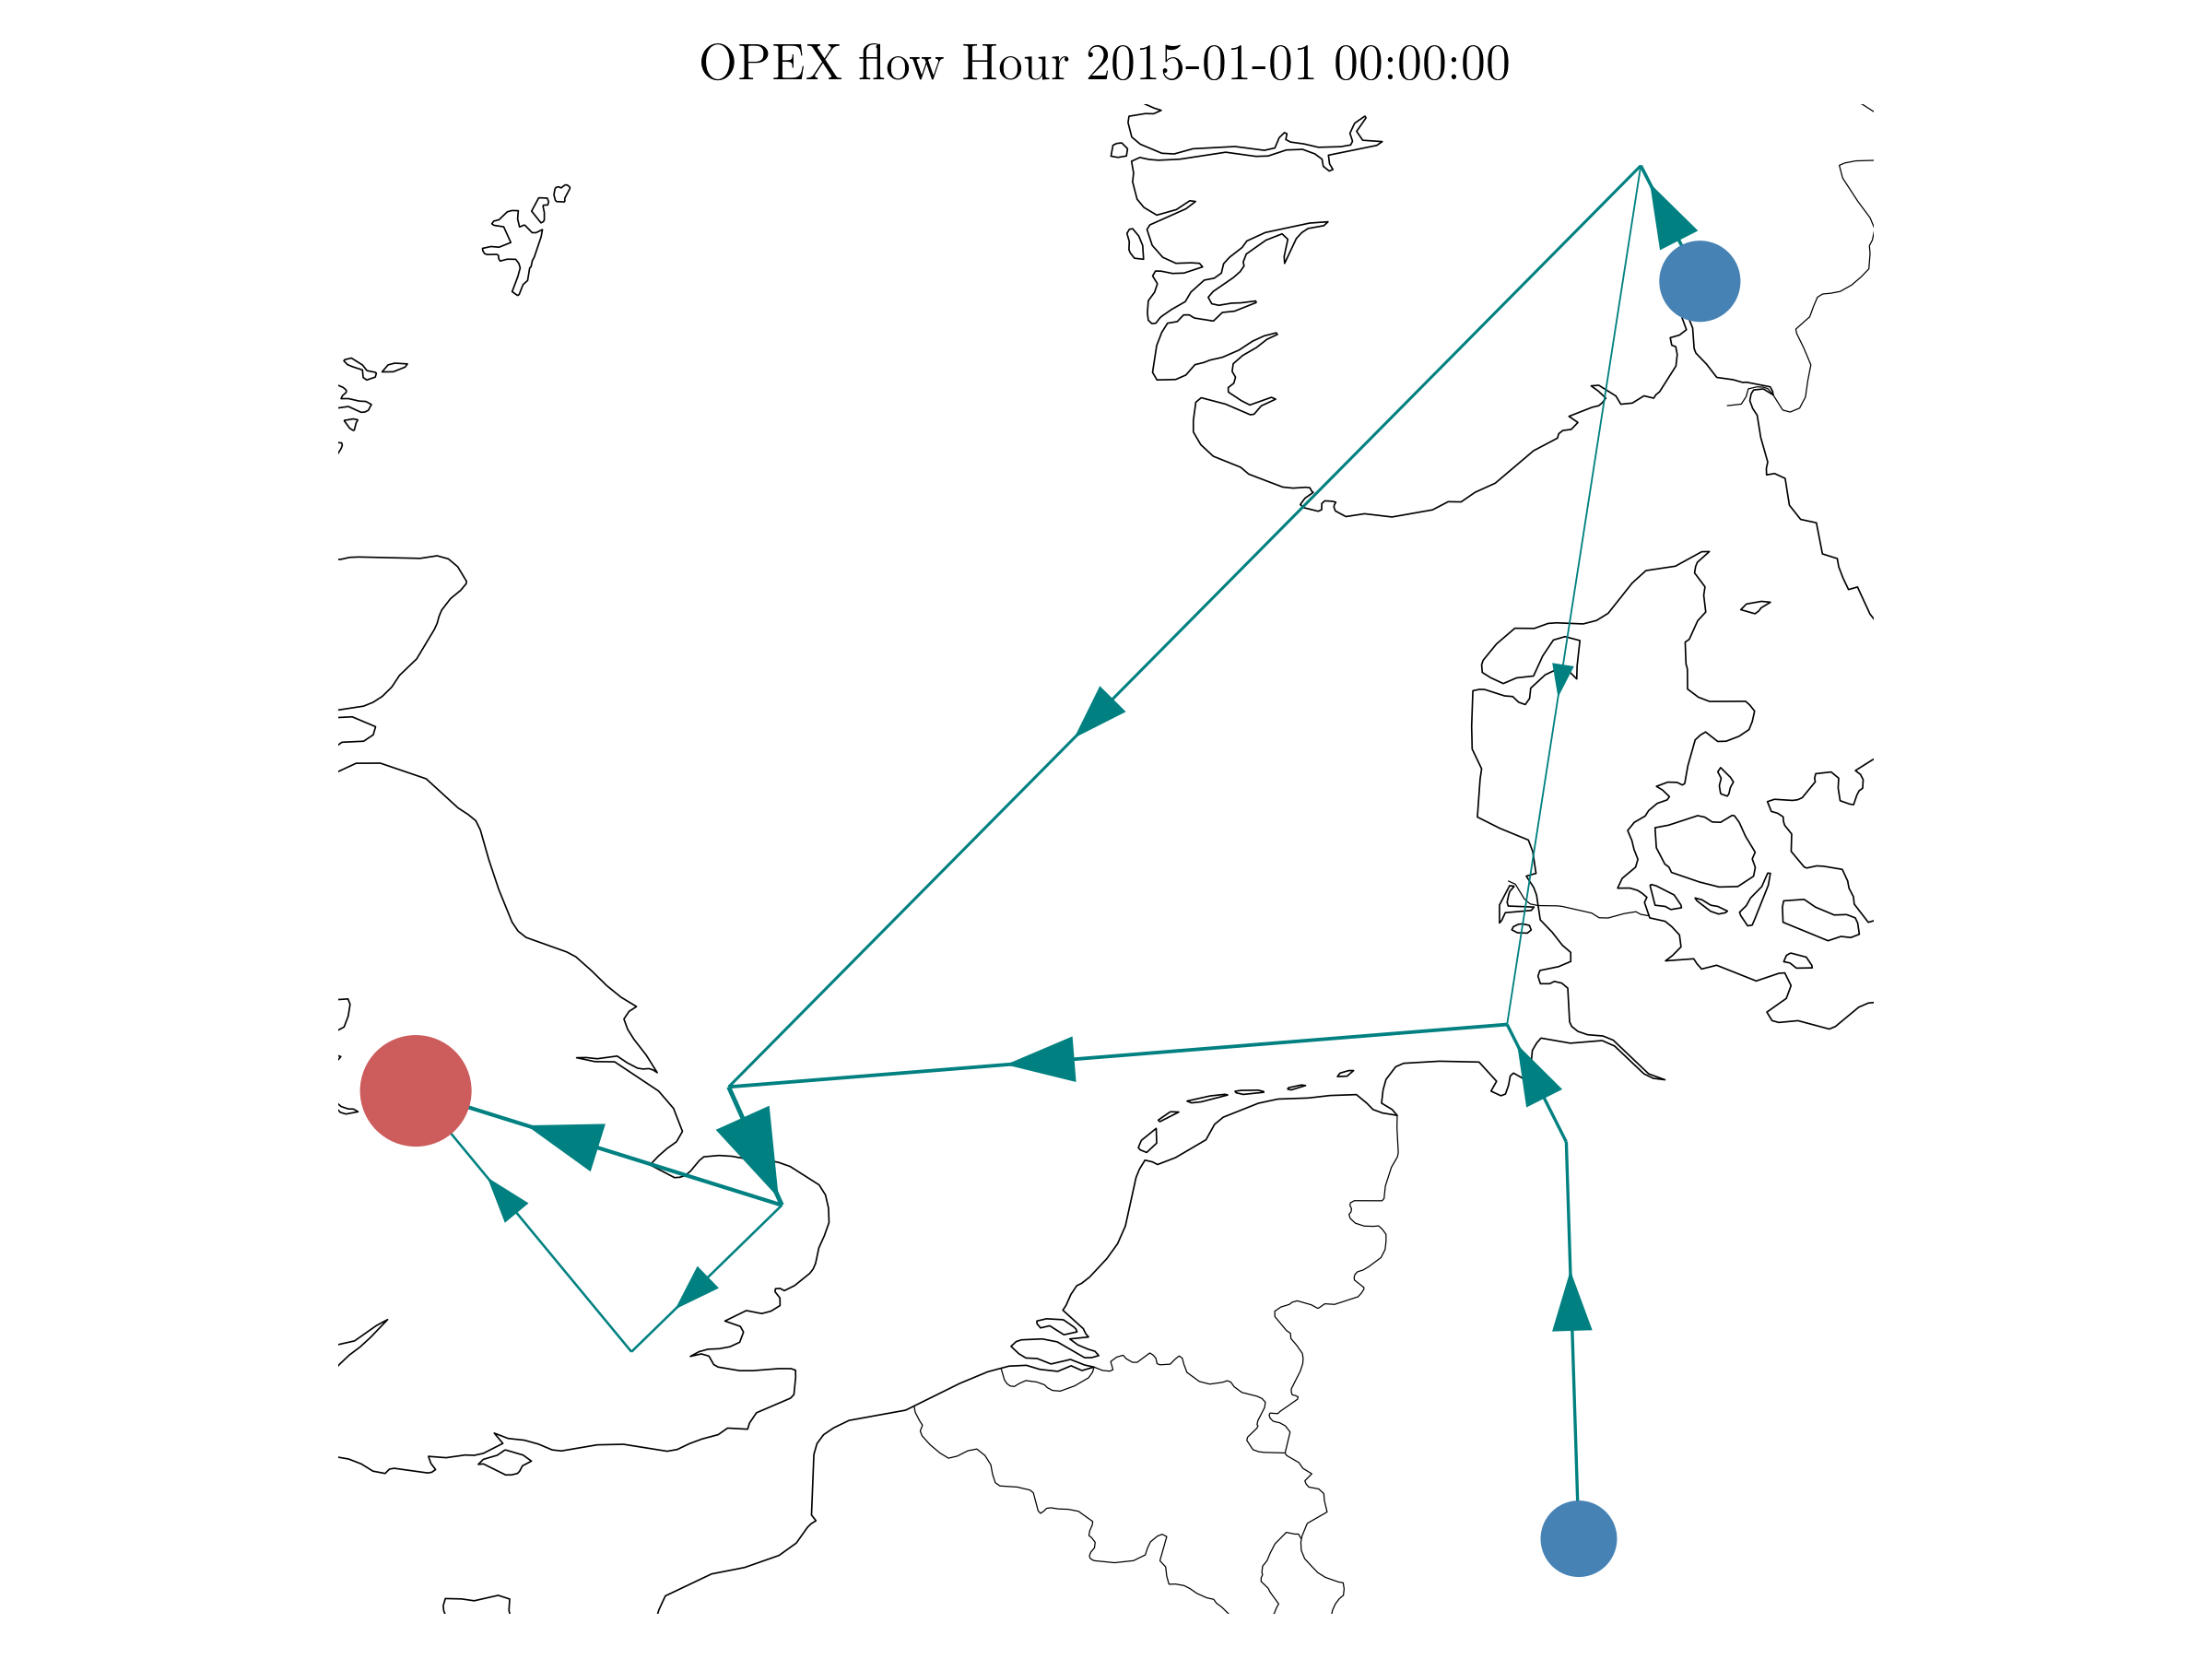
\includegraphics[width=\textwidth]{opex_flow.png}
%       \label{fig:opex_flow}
%     \end{subfigure}%
%     \begin{subfigure}{.5\textwidth}
%       \centering
%       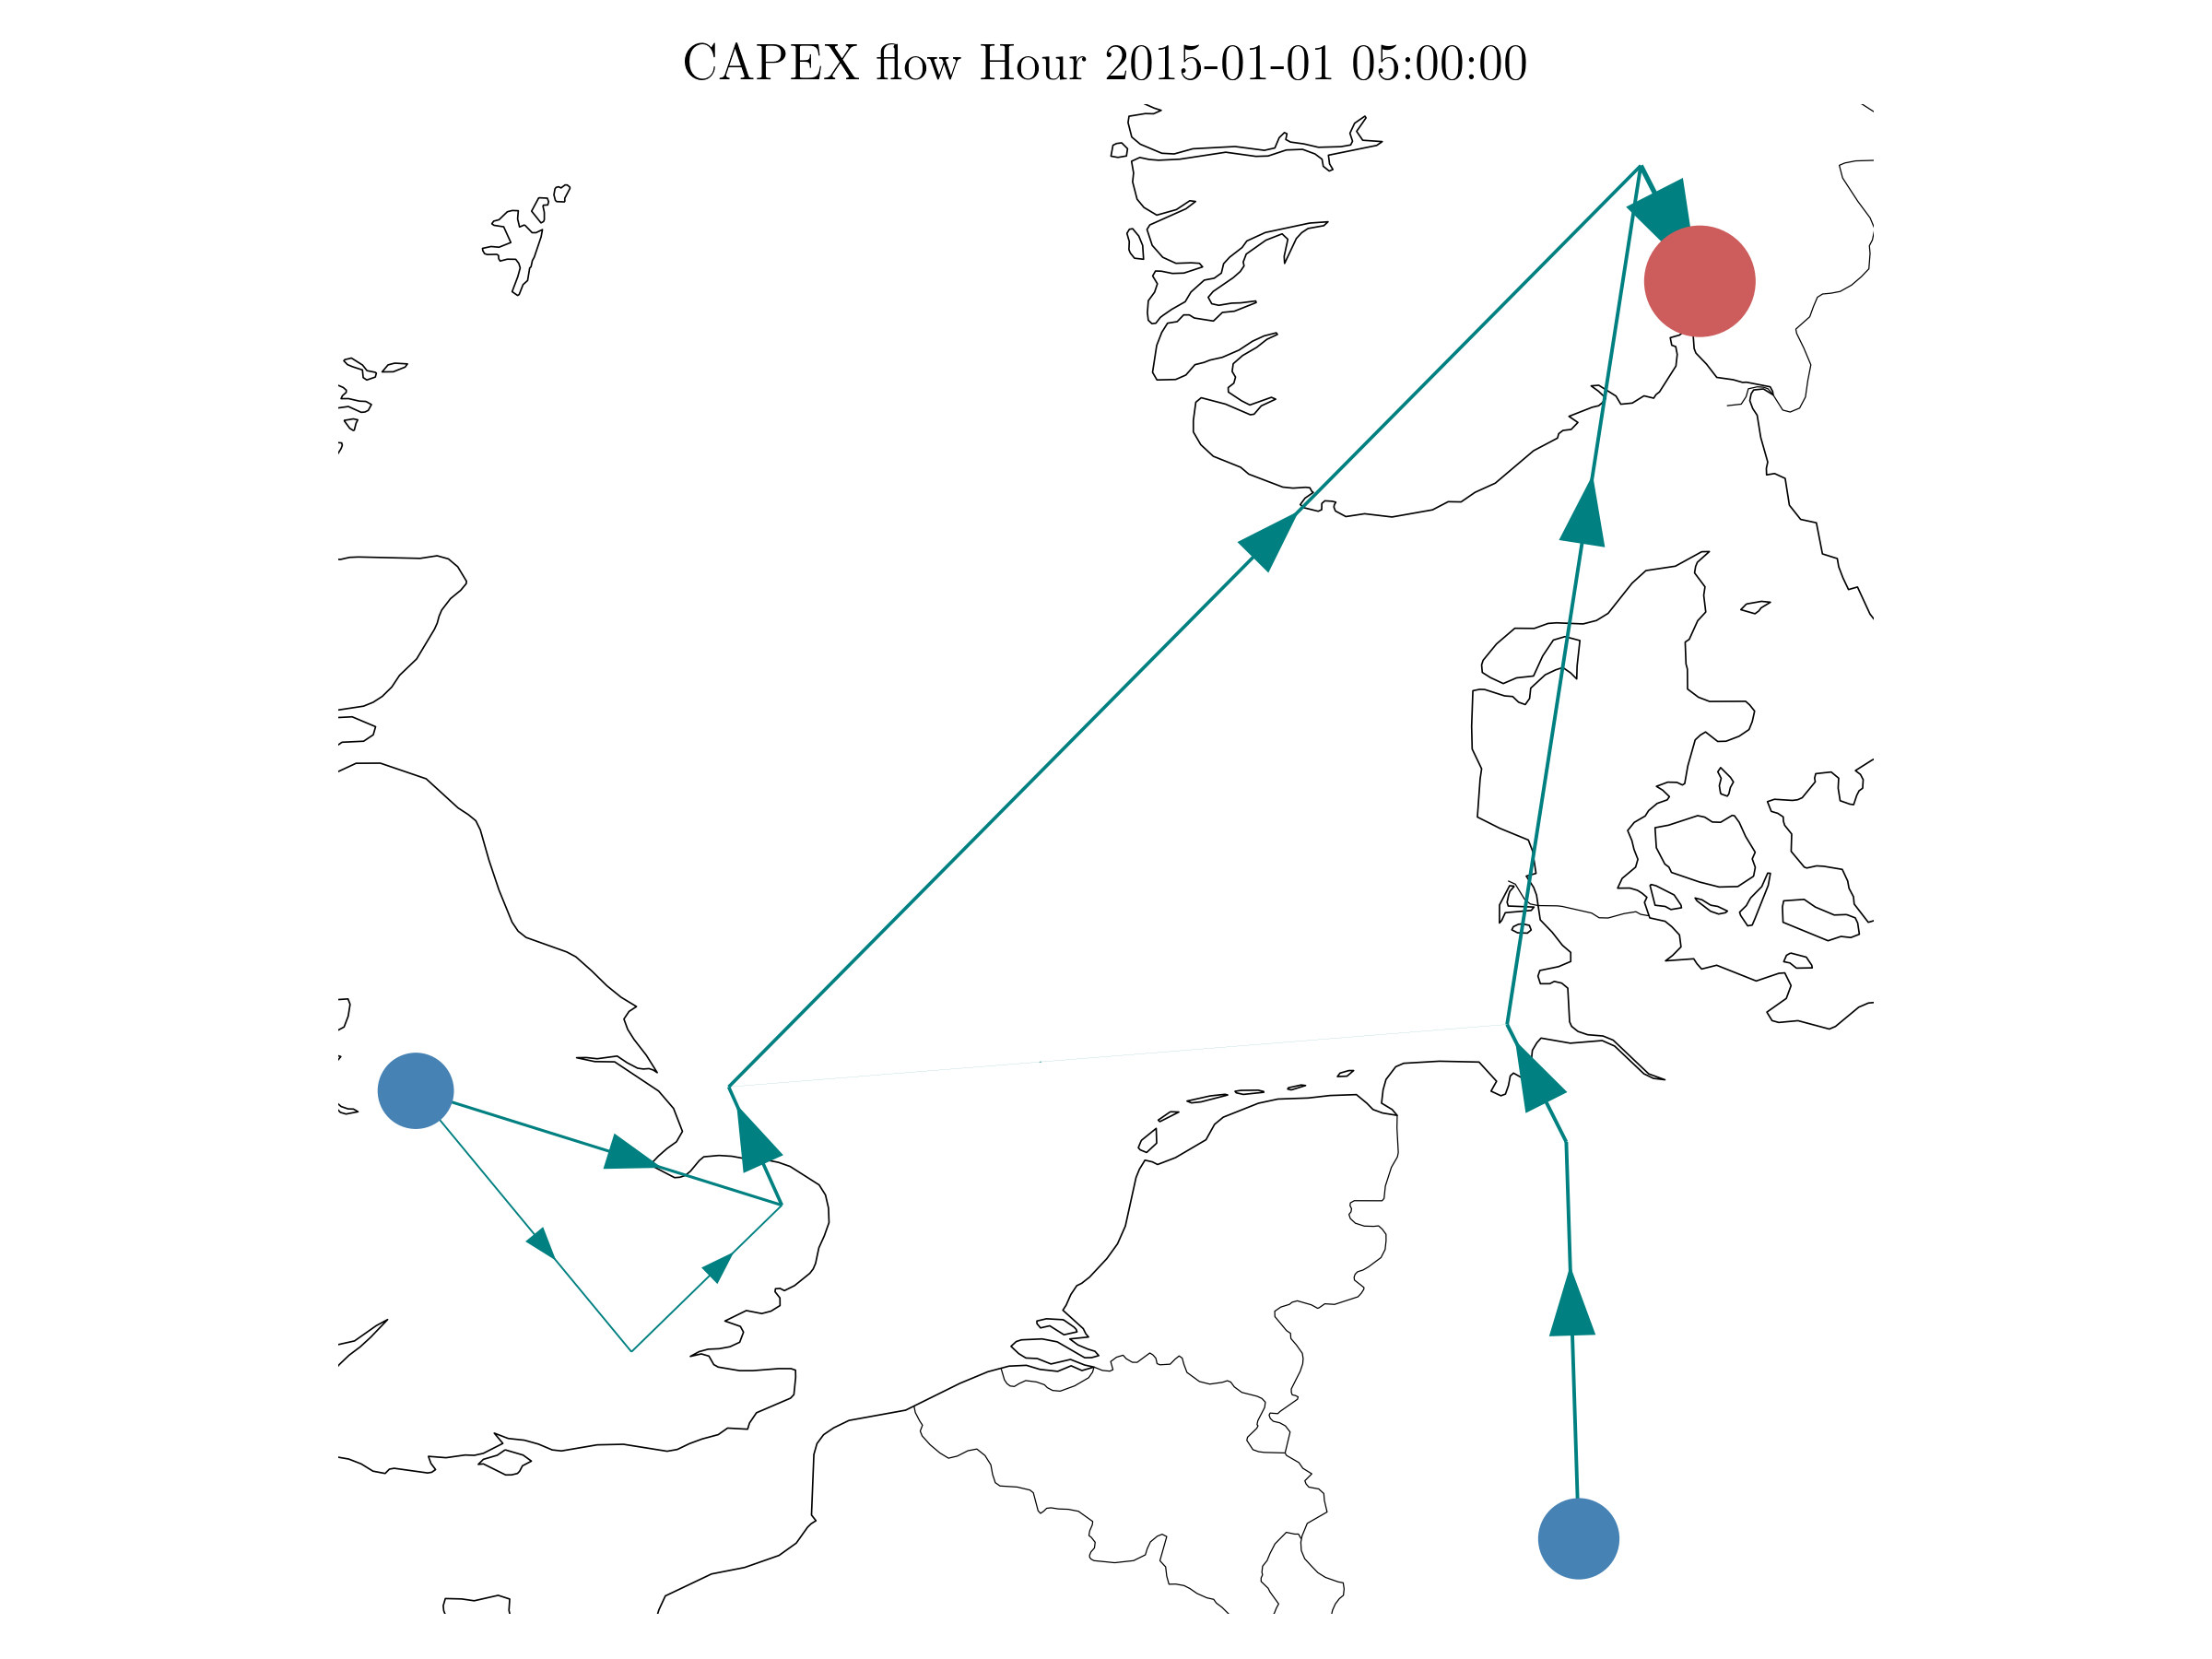
\includegraphics[width=\textwidth]{capex_flow.png}
%       \label{fig:capex_flow}
%     \end{subfigure}
%     \caption{}
%     \label{fig:fig}
% \end{figure}
    
% \begin{appendix}
% Since the P2P comprises all net production and net consumption summing over all sources must result in the nodal demand  
% 
% \begin{align}
%  \sum_{n} \allocatePeer = \sum_a \demand[m]
% \end{align}
% as well as summing over all sinks results in the nodal generation
% \begin{align}
%  \sum_{m} \allocatePeer = \sum_s \generation
% \end{align}
% 
% The P2P relation can be further broke down to allocating generator specific $ \normedgeneration \, \allocatePeer $ where $\normedgeneration = \generation/\sum_s \generation$ denotes the share of generator $s$ of the nodel production. Similarly the allocation to consumers a are given by and consumer specific $ \normeddemand[m] \allocatePeer$ with the nodal comsumer share given by $\normeddemand = \demand/\sum_a \demand$.
% \end{appendix}


% \bibliographystyle{ieeetr}
% \printbibliography


\end{document}
